\chapter{Alternative Models for the Encounter Process}
\label{chapt.poisson-mn}

In the previous chapter we considered a very specific although not
terribly limited observation model. The observation model consisted of
two main elements: First a description of the encounter process 
by which individuals are detected in traps. Specifically, we 
assumed individual trap-specific encounters were iid Bernoulli
trials. The consequence of this is that individuals function
independently of one another and can be captured in
any number of traps during a specific interval of trapping
effort. The type of device is typical of bear hair snares, which we
considered as an example in that section. The 2nd element of the
encounter process model was the specific model – functional form –
relating encounter probability to individual activity center
(``detection probability model'').  It is natural to consider
alternative functional forms of this detection probability model which
we do in Chapt. \ref{chapt.covariates} and elsewhere. 

In this chapter we consider alternative observation models which
accommodate Poisson or multinomial observation models. For example, if
sampling devices can detect an individual some arbitrary number of
times during an interval, then it is natural to consider observation
models for encounter frequencies, such as the Poisson model. Another
type of encounter device is the ``multi-catch'' device (REF XYZ) which
is a physical device that can capture and hold an arbitrary number of
individuals. A typical example is a mist-net for birds 
\citep{borchers_efford:2008}.

We talk about how SCR are multi-state kinds of models. 

We talk about single catch traps. 


\section{Poisson Observation Model}

The models we analyze in Chapt. \ref{chapt.scr0} assumed binary
observations -- i.e., standard encounter history data -- so
that individuals are captured at most one time in a trap.  This makes
sense for many types of DNA sampling (e.g., based on hair snares)
because distinct visits to sampled locations or devices cannot be
differentiated. However, many encounter methods or devices make it
possible to encounter an individual some arbitrary number of times
during any particular sampling episode. That is, we might observe
encounter frequencies $y_{ijk}>0$ 
XXXX DO YOU MEAN $>1$? XXXX
for individual $i$, trap $j$ and
sampling interval $k$.  As an example, if a camera device is
functioning properly it may be programmed to take photos every few
seconds if triggered.  For a second example, suppose we are searching
a quadrat for scat, we may find multiple samples from the same
individual.

Therefore, we seek observation models that accommodate such encounter
frequency data.  Let $y_{ijk}$ be the frequency of encounter for
individual $i$, in trap $j$, during occasion $k$, then a plausible
model is:
\[
 y_{ijk} \sim \mbox{Poisson}(\lambda_{ij})
\]
where the expected encounter frequency $\lambda_{ij}$ depends on both
individual and trap. As we did in the binary model of chapter 4, we
now seek to model the expected value of the observation (which was
$p_{ij}$ in chapter 4) as a function of the individual activity center
${\bf s}_{i}$.
We propose 
\[
 \lambda_{ij} = \lambda_{0}  g({\bf x}_{j},{\bf s}_{i})
\]
Where $g({\bf x},{\bf s})$ is some positive valued function. 
Then $\lambda_{0}g({\bf x},{\bf s})$ is the encounter rate in trap
${\bf x}$ for an individual having activity center ${\bf s}$.  

What does this mean? This means that the encounter rate looks like a
bivariate normal distribution.  
XXXX DOESN'T THIS DEPEND ON THE FORM OF G? XXXX
If we might interpret encounters as
resulting from the outcome of a movement model in the following
sense. Suppose that we telemeter an individual and take measurements
of location sufficiently far apart in time that locations are
independent. Let $x_{t}$ be the location at time $t$. Take a large
number of samples, make a grid and count up the number of observations
in each grid cell.
\[
 E[y(x)] = E[y(x)| moves to x]\Pr(moves to x|s) = \lambda_{0} g(x|s)
\]


For the simplest model in which we have covariates that vary across
the replicate samples $k$, we can aggregate the observed data by the
propetry of compound additivity of the Poisson distribution (if $x$ and
$y$ are $iid$ Poisson with mean $\lambda$ then $x+y$ is Poisson with
mean $2\lambda$). Therefore,
\[
y_{ij} = (\sum_{k=1}^{K} y_{ijk}) =  \mbox{Poisson}(K  \lambda_{0} 
g({\bf x}_{j},{\bf s}_{i}) )
\]
We see that $K$ and $\lambda_{0}$ serve the same role as affecting the
base encounter rate. Since the observation model is the same,
probabilistically speaking, for all values of $K$, evidently we need
only $K=1$ ``survey'' from which to estimate model parameters. We know
this intuitively as sampling by multiple traps serves as replication
in SCR models.


\subsection{Poisson relationship to the Bernoulli model}

There is a sense in which the Poisson and Bernoulli models can
be viewed as consistent with one another. Note that under the Poisson
model we have:
\begin{equation}
 \Pr(y>0) = 1-exp(-\lambda_{0} g({\bf x},{\bf s}))
\label{eq.cloglog}
\end{equation}
Therefore, 
if we equate the event ``encountered'' with the event that the
individual was captured at least 1 time under the Poisson model, i.e., $y>0$, then it would be
natural to set $p_{ij} = \Pr(y>0)$ according to \ref{eq.cloglog}. 

In fact, as $\lambda_0$ gets small, the Poisson model is a close approximation
to the Bernoulli model in the sense that $y$ in that case is almost
always 0 or 1 and, in fact, $\Pr(y>0) \rightarrow \lambda$.  This is
convenient in some cases because the Poisson model might be more
tractable to fit (or even vice versa). For an example, see the models
described in Chapt. \ref{chapt.scr-unmarked}, and we also consider
another case in sec. \ref{XYZ} below.
A plot of that is in order. This near equivalence is shown in  Figure
XYZ. The left panel shows a plot of $\lambda_{ij}$ vs. distance and
superimposed on that is a plot of $p_{ij}$ vs. distance, for values
$\lambda_{0} = .1$ and $\sigma = 1$. The right panel shows a plot of
$\Pr(y>0)$ vs. $E[y]$ and we see therefore that the models are
practically equivalent. 

\begin{verbatim}
x<-seq(0.001,5,,200)
lam0<- .1
sigma<- 1
lam<- lam0*exp(-x*x/(2*sigma*sigma))

par(mfrow=c(1,2))
p1<- 1-exp(-lam)
plot(x,lam,ylab="E[y] or Pr(y>0)",xlab="distance",type="l",lwd=2)
lines(x,p1,lwd=2,col="red")
plot(lam,p1,xlab="E[y]",ylab="Pr(y>0)",type="l",lwd=2)
abline(0,1,col="red")
\end{verbatim}

So under the Poisson model we have
\[
\Pr(y>0) \approx E[y] = \lambda_{0} g(x,s)
\]
whereas in the binary model from chapter 4 we had precisely
\[
\Pr(y>0) \equiv E[y] = p_{0} g(x,s)
\]
and so the models are exactly the same for the {\it expected values}
and very similar for the probability of observing a positive response,
as long as $\lambda_{0}$ is small.


What all of this suggests it that
if we see very few observations $>1$ then we wont lose much
information by using the Bernoulli model. On the other hand, the
Poisson model is more easy to compute in some cases. 


\begin{figure}
\centering
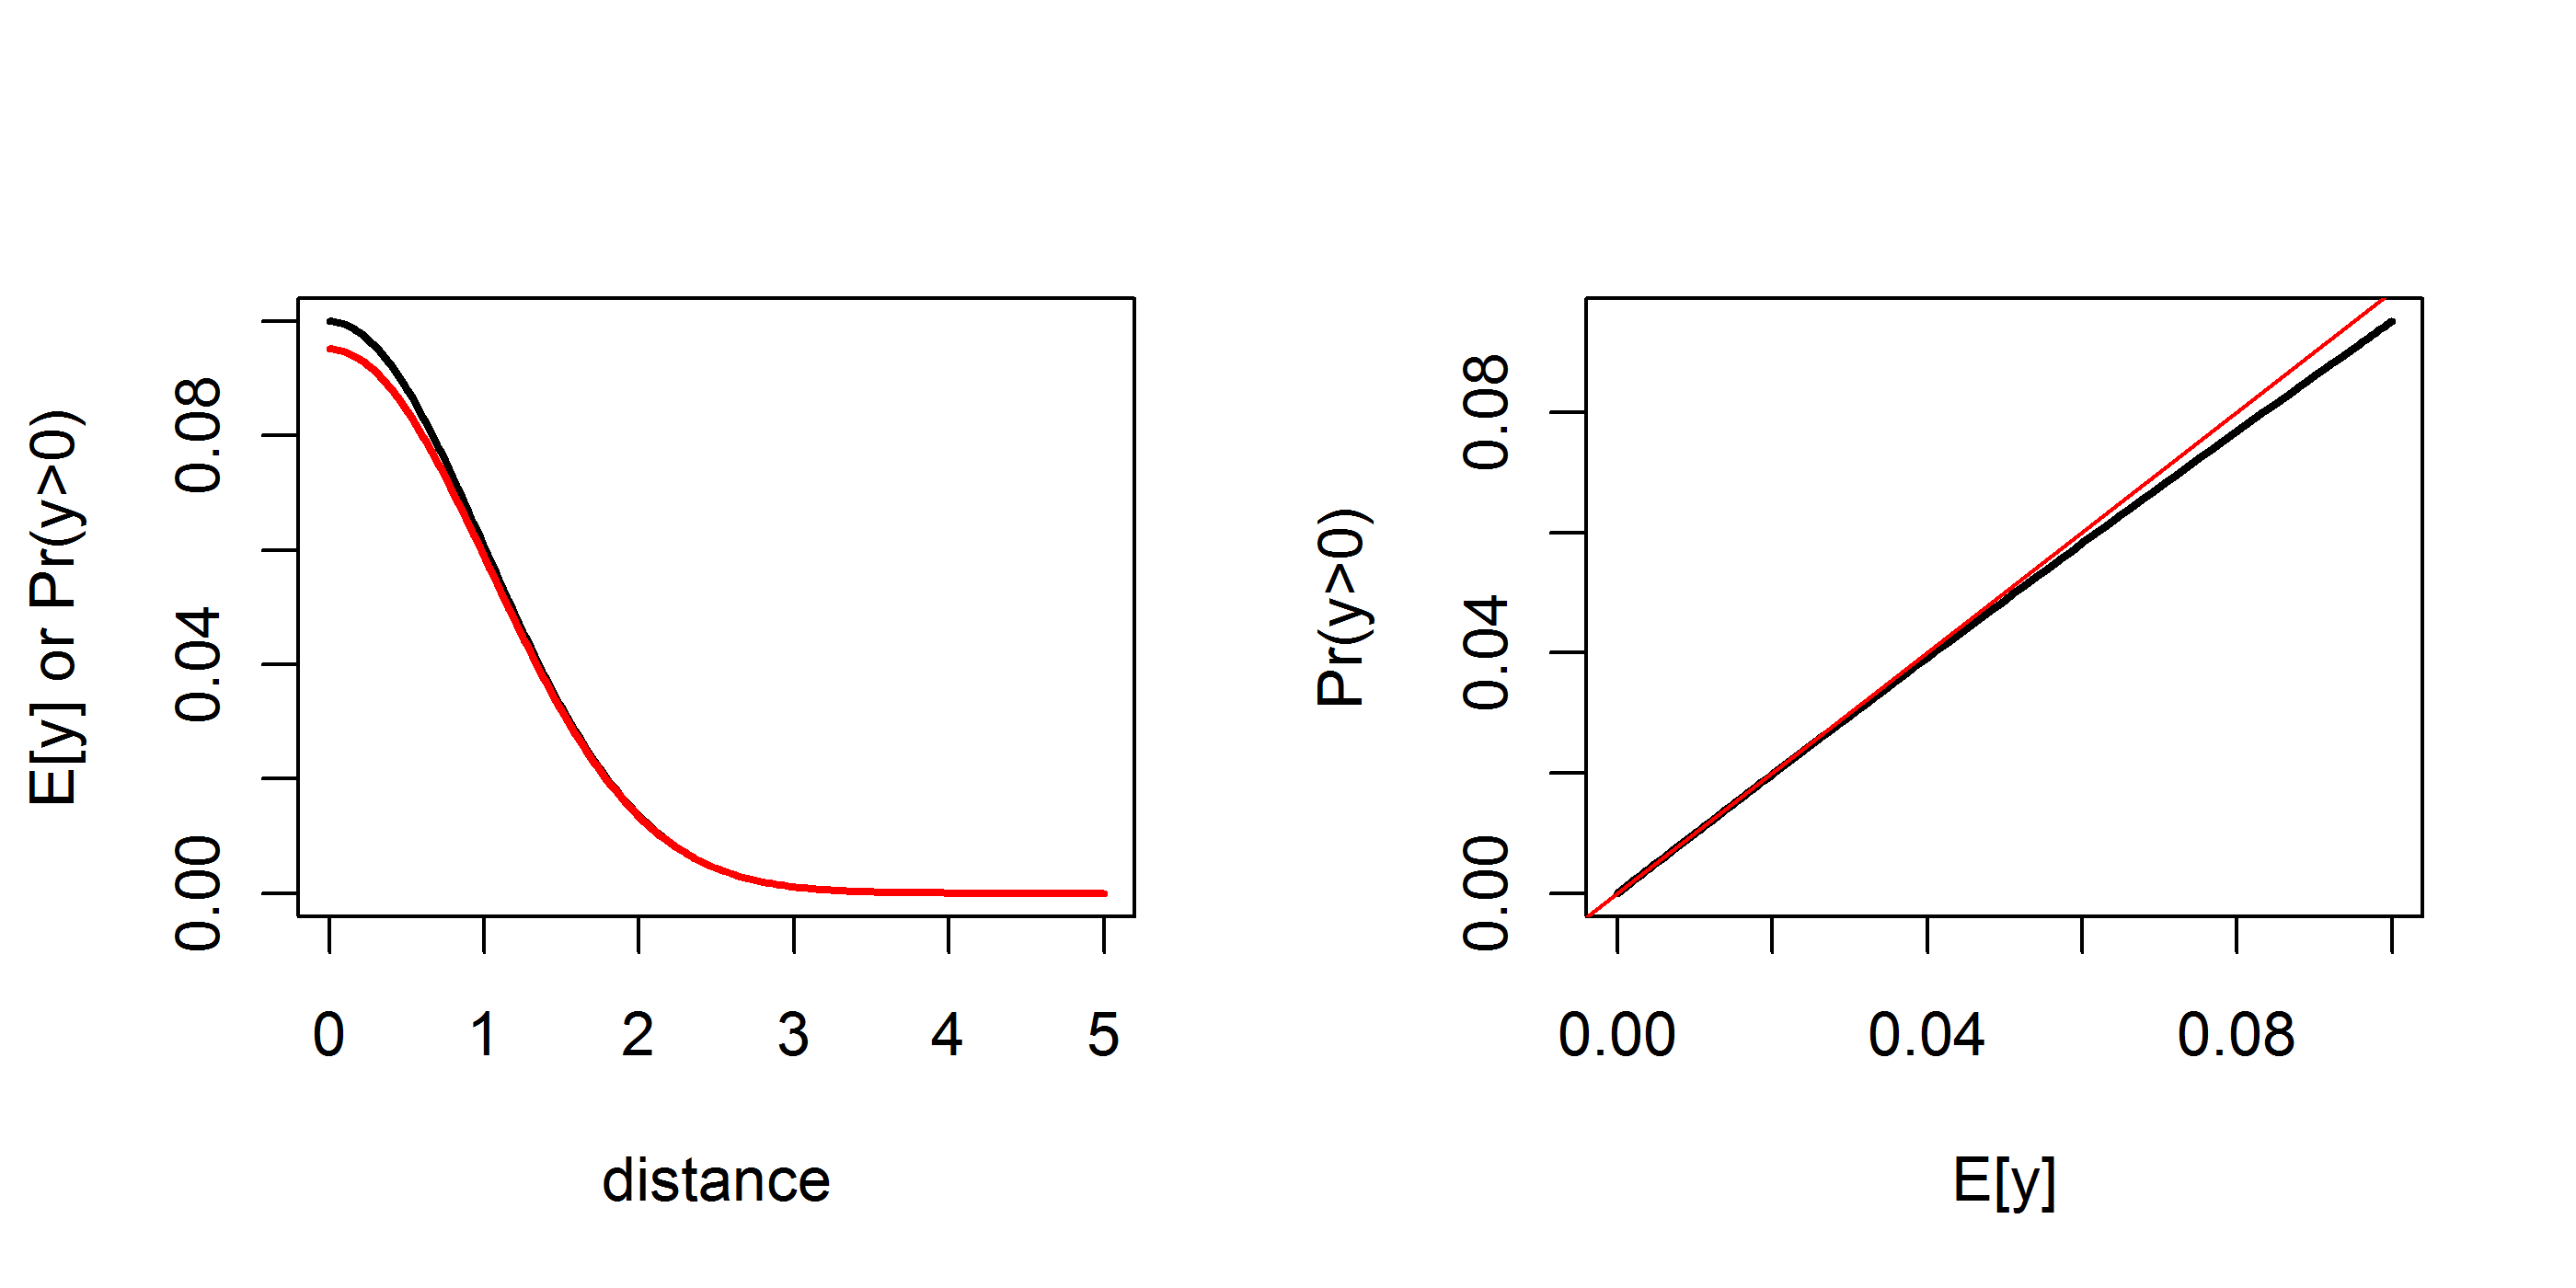
\includegraphics[width=5in,height=2.5in]{Ch5/figs/Poisson-Bern.png}
\label{fig:elevMap}
\end{figure}



Even if we're not in the range where the Bernoulli model provides a
good approximation, we might choose to truncate the counts to binary
observations anyhow (``quantize'').
We might do
this intentionally, but sometimes this truncation is a feature of the
sampling. For example, in the case of bear hair snares, the number of
encounters might be well approximated by a Poisson distribution but we
cannot determine unique visits and so only get to observe the binary
event ``$y>0$''. Similarly for scat sampling problems it will not
generally be possible to diagnose distinct ``independent'' scat
samples. Under this model the data are only binary encounters and we
might therefore choose a model of the form:
\[
 cloglog(p_{ij}) = log(\lambda0)  + log(g({\bf x},{\bf s}))
\]
\begin{comment} 
This example shows us that the choice of link function is typically
directly related to a specific encounter frequency model and,
furthermore, the choice of link function is equivalent to choice of
``detection function.''  As another example, what if the latent
encounter frequencies are actually geometric random variables where
the mean is a function of distance? For the case where the support of
y includes 0 – so that $y$ is the number of failures before the 1st
success, then the mean is $\mu = (1-p)/p$.  $Pr(y>0) =$ ??
\[
logit() = ….?
\]
\end{comment}

\subsection{A cautionary note on modeling encounter frequencies}

Other models for counts might be appropriate. For example, ecologists
are especially fond of negative binomial models for count data
\citep{verhoef_boveng:2007,
white_bennetts:1996,kery_etal:2005}
but other models for excess-Poisson variation are possible. For
example, we might add a normally distributed random effect to
the linear predictor.

As a general rule we favor the Bernoulli observation model even if
encounter frequencies are obtained by sampling.  The main reason is
that, with frequency data, we are forced to confront a model choice
problem (i.e., Poisson, negative binomial, log-normal mixture) that is
wholly unrelated to the fundamental space usage process that underlies
the genesis of SCR data. Repeated encounters over short time intervals
are not likely to be the result of independent encounter
processes. E.g., an individual moving back and forth in front of a
camera yields a cluster of observations that is not informative about
the spatial structure of the model. Similarly in scat surveys (e.g.,
Thompson et al. in review), dogs are used to locate scats which are
processed in the lab for individuality.  The process of local scat
deposition is not really the outcome of movement but rather the
outcome of complex behavioral considerations as well as dependence in
detection of scat by dogs. E.g., they find one and then more likely to
find a nearby one, or they get into a den area and find lots of scats.
This additional model assumption required to model variation in
observed frequencies (i.e., conditional on location) provides
relatively little information about density, and we feel that the
model selection issue should therefore be avoided.

To elaborate on this, it seems natural to construct models for
encounter data that is conditional on movement outcomes: We suppose
that an individual visits a particular location with some probability
$p_{ik}$ say $z_{ik}\sim  \mbox{Bern}(p_{ik})$ and then deposits a number of scat,
or visits a camera some number of times with frequency $y_{ik}$ which
is 
an integer $> 0$. Therefore, a sensible model might be
$[y|z][z|\phi({\bf x},{\bf s})$
XXXX THIS NOTATION DIFFERS FROM THAT GIVEN ABOVE XXXX
where the encounter frequency $y$ is independent of ${\bf x}$ and
${\bf s}$ conditional
on the binary event ``$z$'' that the individual visited the vicinity of
the trap.

Moreover, consideration of encounter frequency data could lead to
important identifiability problems along the lines of \citet{link:2003}. The
basic Poisson model can be over-dispersed in a number of ways to
produce different models of over-dispersion.  i.e., gamma noise,
normal noise, exponential noise, etc..  Thus we have different models
of heterogeneity analogous to the class of models considered by \citet{link:2003}.


\section{Analysis of a Poisson SCR model in BUGS}

We consider the simplest possible model here in which we have no
covariates that vary over replicate samples $k$ so that we work with
the aggregated individual- and trap-specific encounters:
\[
y_{ij} = (\sum_{k=1}^{K} y_{ijk}) =  \mbox{Poisson}(K  \lambda_{ij})
\]
We consider a bivariate normal form of $g({\bf x}_{j},{\bf s}_{i})$ so
that
\[
g({\bf x}_{j},{\bf s}_{i}) = exp( -||{\bf x}_{j} - {\bf
  s}_{i}||^{2} /(2\sigma^{2}))
\]
In this case, note that 
\[
log( \lambda_{ij})  =\alpha_{0} - \beta ||{\bf x}_{j} - {\bf s}_{i}||^2
\]
where $\alpha_{0} = log(\lambda_{0})$ and $\beta = 1/(2\sigma^2)$.


As usual, we approach Bayesian analysis of these
models using data augmentation (section \ref{closed.sec.da}). 
It is interesting in this case that DA
gives us a sort of zero-inflated Poisson model which is amazingly easy
to analyze by likelihood methods which maybe we will do in Chapter
XYZ.

So the model specified conditional on $z_{i}$ is
\[
y_{ij} \sim  Poisson(z_{i} K  \lambda_{ij})
\]
which evaluates to a point mass at $y=0$ if $z=0$. 


\subsection{Simulating Data}

Simulating a sample SCR data set under the Poisson model requires only
a couple minor modifications to the procedure we used in chapter 4. In
particular, we modify the block of code which defines the model to be
that of $E[y]$ and not $\Pr(y=1)$, and we change the random variable
generator from \mbox{\tt rbinom} to \mbox{\tt rpois}:
\begin{verbatim}
D<- e2dist(S,traplocs)

alpha0<- -2.5
sigma<- 0.5
beta<- 1/(2*sigma*sigma)

muy <-  exp(alpha0)*exp(-beta*D*D)
# now generate the encounters of every individual in every trap
Y<-matrix(NA,nrow=N,ncol=ntraps)
for(i in 1:nrow(Y)){
 Y[i,]<-rpois(ntraps,K*muy[i,])
}
\end{verbatim}

We modified our code from SCR0 in chapter 4 to simulate Poisson
encounter frequencies for each trap and then we analyze an ideal data
set using WinBUGS. The new function, available in the R package, is called
{\tt simPoissonSCR.fn}. 
The simulator can produce 3-d encounter history data too although we
don't do that here. 
Here is an example of simulating a data set and harvesting the
required data objects:

\begin{verbatim}
data<-simPoissonSCR.fn(discard0=TRUE,sd=2013)
y<-data$Y
traplocs<-data$traplocs
nind<-nrow(y)
X<-data$traplocs
K<-data$K
J<-nrow(X)
Xl<-data$xlim[1]
Yl<-data$ylim[1]
Xu<-data$xlim[2]
Yu<-data$ylim[2]

## Data augmentation stuff
M<-200
y<-rbind(y,matrix(0,nrow=M-nind,ncol=ncol(y)))
z<-c(rep(1,nind),rep(0,M-nind))
\end{verbatim}

To execute WinBUGS the process is identical to what we've done
previously..............................................
here..................
.................................

The results are given below. We note about the same answer as before.

{\small
\begin{verbatim}
> print(out1,digits=2)
Inference for Bugs model at "SCR-Poisson.txt", fit using WinBUGS,
 3 chains, each with 2000 iterations (first 1000 discarded)
 n.sims = 3000 iterations saved
           mean    sd   2.5%    25%    50%    75%  97.5% Rhat n.eff
alpha0    -2.57  0.19  -2.95  -2.69  -2.57  -2.44  -2.19 1.00  2600
beta       2.34  0.36   1.69   2.08   2.32   2.57   3.12 1.00  3000
N        114.13 15.25  87.97 103.00 113.00 124.00 147.00 1.01   370
D          1.78  0.24   1.37   1.61   1.77   1.94   2.30 1.01   370
deviance 329.95 21.92 290.00 314.20 329.50 344.40 375.80 1.00  1700

For each parameter, n.eff is a crude measure of effective sample size,
and Rhat is the potential scale reduction factor (at convergence, Rhat=1).

DIC info (using the rule, pD = var(deviance)/2)
pD = 240.2 and DIC = 570.2
DIC is an estimate of expected predictive error (lower deviance is better).
\end{verbatim}


At the end of this chapter we provide an example of a Poisson SCR model fitted to 
real data. This example has some other features which we encounter before
arriving there. 

\subsection{Exercise}

Use the Bernoulli model simulator from Chapt. \ref{chapt.scr0} (\mbox{\tt
  simSCR0.fn}) to simulate a Bernoulli data set and then fit the
Poisson model. Compare the results of fitting the correct
data-generating model with those of fitting the misspecified Poisson
model. 



\begin{comment}
\section{Likelihood analysis of the Poisson model}

Counts are Poisson with a random effect so this is stupidly easy to
implement. 
We do the normal ``full likelihood'' approach in which we retain $N$
as a real parameter in the model. We adapt \mbox{\tt intlik3} from
chapter 5 here..... behold:

Poisson(lambda(s,x))

data augmentation = ZIP
\begin{verbatim}
Pr(yi) =   ( prod_{j} dpois(y) ) *psi + I(y=0)*(1-psi)

Actually if y(i,j) = Poisson( lambda(i,j) ) then we can just add up
sum_{j} y(i,j) =  Poisson( sum_{j} lambda(i,j)) right?

 int_{s} thatthing

Zero-inflate the result
\end{verbatim}
\end{comment}

\section{No real example}

In chapt. \ref{chapt.searchencounter} we analyze the cap crap data.


\section{Independent Multinomial Observations}

Several types of encounter devices yield multinomial observations in
which an individual can be caught in a single trap during a particular
encounter occasion.  Mist nettting is a major example -- these are
``multi-catch'' traps (Efford XYZ NEED REF HERE XXXX). Also some kinds of
mammal traps hold multiples of animals and can be thought of
similarly. Another one is area-searches of reptiles where we think of
a small polygon as the ``trap'' -- we could get multiple individuals
(turtles, lizards) in the same plot but not, in the same sample
session, at different plots.  The key feature is that capture of an
individual in a trap is {\it not} independent of capture in other
traps, because they can't be captured once they are captured. On the
other hand individuals behave independently of one another, or so it
might be reasonable to assume, so whether a trap captures some other
individual doesn't have bearning on whether it captures another.  This
last assumption is violated in an extreme case in classical ``single
catch'' traps which we address in section \ref{poisson-mn.sec.singlecatch}
below. In general we could imagine non-independence being important in
any multi-catch situation but to the best of our knowledge a general
model that encompasses complete dependence (single catch) and complete
independence (multi-catch) of individuals has not been proposed.  So
we treat the cases individually and, in this section, we address the
multi-catch situation wherein individuals behave independently.


In this case we regard the observation ${\bf y}_{ik}$ for
individual $i$ during sample occasion $k$ as a multinomial observation
which consists of a sequence of 0's and at most a single 1 indiciating
the trap of capture. For example, if we capture an individual in trap
2 during a 6 sample period study then ${\bf y}_{i} = (0,1,0,0,0,0)$.
If we sample for 5 periods in all and the individual is also caught
in trap 4 during sample 3, then the 5 encounter observations for that
individual are as follows:
\begin{verbatim}
sample |---- trap ---------|
       1   2   3   4   5   6
 1     0   1   0   0   0   0
 2     0   0   0   0   0   0
 3     0   0   0   1   0   0
 4     0   0   0   0   0   0
 5     0   0   0   0   0   0
\end{verbatim}
Statistically we regard the {\it rows} of this data matrix as {\it
  independent} multinomial trials.

Analogous to our previous Bernoulli and Poisson models, we seek to
construct the multinomial cell probabilities for each individual, as a
function of {\it where} that individual lives, through its center of
activity ${\bf s}$. Thus we suppose that
\[
 {\bf y}_{ik} \sim \mbox{Multinom}(1, {\bm \pi}({\bf s}_{i}) )
\]
where ${\bm \pi}({\bf s}_{i})$ is a vector of length $J+1$, which, by
convention here, we define $\pi_{i,J+1}$, the last cell, or the ``zero
cell'', to correspond to the event ``not captured''.  Now we have to
construct these cell probabilities in some meaningful way that depends
on each individuals' ${\bf s}$, which we do shortly.

A statistically equivalent distribution is the {\it categorical} distribution.
If ${\bf y}$ is a multinomial trial with probabilities
${\bm \pi}$ than the {\it position} of the non-zero
elemment of ${\bf y}$ is a categorical random variable with probabilities
${\bm \pi}$.
We express this as
\[
{\bf y} \sim \mbox{Categorical}( {\bm \pi} )
\]
In the context of SCR models the categorical version of the
multinomial trial corresponds to the {\it trap of capture}.  Using our
example above with 6 traps then ${\bf y}_{i1} = (0,1,0,0,0,0)$ then we
could as well say $y_{ik}$ is a categorical random variable with
possible outcomes $(1,2,3,4,5,6,7)$ where outcome $y=7$ corresponds to
``not captured'' (obviously how this is organized or labeled is
completely irrelevant, although it is convenient to use the integers
$1:(J+1)$).  Therefore, $y_{i1} = 2$, $y_{i2} = 7$, $y_{i3} = 4$ and
so on.

For simulating and fitting data in the {\bf BUGS} engines we will typically use
the categorical representation of the model because it is somewhat
more convenient.  We have found that fitting multinomial models in
{\bf WinBUGS} can be extremely inefficient whereas {\bf JAGS}
typically performs much better. In the examples here, we use {\bf
  JAGS} exclusively.

\subsection{Multinomial Relationship to Poisson}

The multinomial is related directly to the Poisson encounter rate
model in the following sense. Let $y_{ij}$ be the total number of
encounters for individual $i$ in trap $j$. Then, the trap frequencies
(excluding the last cell now), if we condition on the {\it total}
number of captures, $y_{i} = \sum_{j} y_{ij}$, are multinomial with
probabilities
\[
 \pi_{ij} =  \frac{ \lambda_{ij} } { \sum_{j} \lambda_{ij} } 
\]
for $j=1,2,\ldots,J$.
Or equivalently the {\it trap of
  capture} is categorical with probabilities
\[
 \pi_{ij} =  \frac{ \lambda_{ij} } { \sum_{j} \lambda_{ij} } 
\]
which is precsely, under the half normal model, 
\[
 \pi_{ij} =  \frac{ \exp( - \beta \! dist({\bf x},{\bf s})^2 ) }  {
   \sum_{j} \exp(-\beta \! dist({\bf x},{\bf s})^2)}
\]
This expression looks like a multinomial inverse-logit transform of a model having
quadratic distance term, and also ``maximum entropy'' from MAXENT
species distribution modeling, or resource utilzation distribution
from telemetry studies.
So we can think of this multinomial model as arising naturally 
by having Poiosson encounters and then conditioning on the total. 
It is a sensible model to have anyhow, as it just allocates captures
to traps in proportion to the square of distance.  We could try other
models here too (Note: What do Borchers and Efford 2008 do?).

%People might think this multinomioal model is somehow more general
%than assuming Poisson encounter frequencies since we might cook up the
%multinomioal without having to specify a distribution for
%$y_{i}$. That said, we note that it arises under 
%If we now uncondition on the total..... 
%$y_{ij}$ is Poisson with mean $\sum_{j}$ stuff... we have a product of
%Poissons, i.e., the model we started with. 

The interpretation of this model merits some discussion. That is, 
{\it given that an individual is captured}, the probabilities given by
eq. XYZ determine 
the distribution among traps. To fully specify the model, we have to
model the probability that an individual is captured, say $p$.

We deduced the multinomial by assuming a Poisson distribution
..... so
where did this $p$ come from?

So lets not worry about the distribution of the total count
but instead estimated this excess parameter p (this is what Royle et al.
and Gardner et al. tried to do).  In this case the multinomial gets
another cell probability , the J+1 cell, 
\[
 \pi\_{ij} =  \frac{ p exp( - beta d^2 ) }  { \sum\_{j} exp(-beta d^2)}
\]
and the last cell
\[
 \pi\_{i,J+1} =  1-p 
\]

What i like about this particular multiomial model is that whether or not
an individual is encounter in trap $j$ is just a Bernoulli trial with
probability
\[ 
(p/stuff)*exp(-beta*d^2)
\]
and if we just label (p/stuff) = p0 then this is precisely our
Bernoulli model with a half-normal detection model.  Thus we ``condition''
on $y_{ij}$ and we dont have to fess up to a model for this encounter
rate, which is most of the time just reflecting behavioral stuff of the
species under, study and we wind up with a basic default Bernoulli model
which doesn't require any assumptions about the encounter rate of 
individuals.  So not having to model encounter rate seems like a good
benefit of the Bernoulli model -- which is why we said what we did above.


\subsection{Simulating data and fitting in WinBUGS}

We're going to show the nugget of a simulation function which is
used in the function \mbox{\tt sim.mnSCR} found in the {\bf R} package
\mbox{\tt scrbook}.  The first lines of the following {\bf R} code
make use of some things that should be defined but we omit them here:
{\small
\begin{verbatim}
S<-cbind(runif(N,Xl,Xu),runif(N,Yl,Yu))
# how far is each individual from each trap?
D<- e2dist(S,traplocs)

# paramter values
sigma<- 0.5
alpha0<- -1
theta<- 1/(2*sigma*sigma)

# make an empty data matrix and fill it up
Ycat<-matrix(NA,nrow=N,ncol=K)
for(i in 1:N){
for(k in 1:K){
lp<- alpha0 - theta*D[i,]*D[i,]
cp<- exp(c(lp,0))
cp<- cp/sum(cp)
Ycat[i,k]<- sample(1:(ntraps+1),1,prob=cp)
}
}
\end{verbatim}
}
The resulting data matrix in this case has the maximal dimension $N$
and so, for analysis, to mimic a real situation, we would have to discard the uncaptured
individuals. 
\mbox{\tt sim.mnSCR} will also simulate data that includes a
behavioral response, which will be the typical situation in
small-mammal trapping problems, which we first developed this code to
deal with \citep[see][for details]{converse_royle:2012}.

Here we use our function \mbox{\tt sim.mnSCR} to simulate a data set
with $K=7$ periods, etc.. We'll run the model using {\bf JAGS} which we
have found is much more effective for this class of models.
We get the data set-up for analysis by augmenting the size of the data
set to $M=200$. In addition we choose starting values for ${\bf s}$ and the
data augmentation variables $z$.  For ${\bf s}$ here we cheat a little bit
and use the true values for the obseved individuals and then augment
the matrix ${\bf S}$ with $M-n$ randomly selected activity centers.

{\small 
\begin{verbatim}
set.seed(2013)
parms<-list(N=100,alpha0= -.40, alpha1= 0,sigma=0.5)
data<-sim.mnSCR(parms,K=7,ssbuff=2)
nind<-nrow(data$Ycat)

M<-200
Ycat<-rbind(data$Ycat,matrix(nrow(data$X)+1,nrow=(M-nind),ncol=data$K))
Sst <-rbind(data$S,cbind(runif(M-nind,data$xlim[1],data$xlim[2]),
                         runif(M-nind,data$ylim[1],data$ylim[2])))
zst<-c(rep(1,160),rep(0,40))
\end{verbatim}
}

The model specification is not much more complicated than the binomial
or Poisson models given previously. The main consideration is that we
define the cell probabilities for each trap $j=1,2,\dots,J$ and then
define the last cell probability, $J+1$, for ``not captured'', to be
the complement of the sum of the others. The code is shown in Panel
\ref{poisson-mn.panel.mn}.
In the last lines of code here we
specify $N$ and density, $D$, as  derived parameters.


\begin{panel}[htp]
\centering
\rule[0.15in]{\textwidth}{.03in}
%\begin{minipage}{2.5in}
{\small
\begin{verbatim}
cat("
model {
psi ~ dunif(0,1)
alpha0 ~ dnorm(0,10)
sigma ~dunif(0,10)
theta<- 1/(2*sigma*sigma)

for(i in 1:M){
  z[i] ~ dbern(psi)
  S[i,1] ~ dunif(xlim[1],xlim[2])
  S[i,2] ~ dunif(ylim[1],ylim[2])
  for(j in 1:ntraps){
    #distance from capture to the center of the home range
    d[i,j] <- pow(pow(S[i,1]-X[j,1],2) + pow(S[i,2]-X[j,2],2),1)
  }
  for(k in 1:K){
    for(j in 1:ntraps){
      lp[i,k,j] <- exp(alpha0 - theta*d[i,j])*z[i]            
      cp[i,k,j] <- lp[i,k,j]/(1+sum(lp[i,k,]))
    }
    cp[i,k,ntraps+1] <- 1-sum(cp[i,k,1:ntraps])  # last cell = not captured
    Ycat[i,k] ~ dcat(cp[i,k,])
  }  
}   

N <- sum(z[1:M]) 
A <- ((xlim[2]-xlim[1])*trap.space)*((ylim[2]-ylim[1])*trap.space)
D <- N.tot/A
}
",file="model.txt")

\end{verbatim}
}
%\end{minipage}
\rule[-0.15in]{\textwidth}{.03in}
\caption{
WinBUGS model specification for the multinomial observation model. 
}
\label{poisson-mn.panel.mn}
\end{panel}

Finally we need to package everything up (inits, parameters, data) and send
it off to {\bf JAGS} to build a MCMC simulator for us:

{\small
\begin{verbatim}
library("rjags")

inits <- function(){list (z=zst,sigma=runif(1,.5,1) ,S=Sst) }              
parameters <- c("psi","alpha0","theta","sigma","N","D")
data <- list (X=data$X,K=data$K,trap.space=1,Ycat=Ycat,M=M,
              ntraps=nrow(data$X),ylim=data$ylim,xlim=data$xlim)         

out1 <- jags.model("model.txt", data, inits, n.chains=3, n.adapt=500)
out2 <- coda.samples(out1,parameters,n.iter=1000)
\end{verbatim}
}


Summary of analysis for the simulated data set here.....  



\section{ Mist-netting example}

Here we do an analysis of a real data set using the multinomial model.
the data are for 
adult Arctic Warblers ({\it Phylloscopus borealis}) banded 
 along the Colville River near Umiat, Alaska in 2006. The data are from 
 5 MAPS (REF) stations located in close proximity of one another, as
 well as 
 birds target (netids starting with "UMIA") or passive (netids starting 
 with "PASS") netted in the general area (a couple of nets, 
 netid == 'PASS01' and 'UMIAB3' are pretty far away though...). In total, 
 there are 258 captures of 179 individual birds. This is is really a 
 large number of birds of a single species for MAPS stations. 
 
Each of these MAPS stations has 12-15 nets.

We used XYZ....
 
A few issues:
 data is manipulated into multinomial trials and we have to convert.
 multiple captures somehow.....
 lots of space.
 transient individuals?  affect is N = number of guys ``ever available''
 


\section{SCR Models are Multi-State Models}

\begin{comment}
SCR models are multi-state models where stat-especific encounter
probabilities are a function of distance -- or something like that. 
\end{comment}

This multinomial observation model and also the discrete formulation
of the state-model given in section XYZ both allude to the fact that
SCR models are a variation of 
ordinary multi-state models \citep[][Chapt. 9]{kery_schaub:2011}
but where the state variable is static and represents a
geographic location. Multi-state models are extremely useful for
modeling movements among geographic states and indeed this type of
problem motivated their early developments by
\citet{arnason:1972,arnason:1973} and 
\citet{hestbeck_etal:1991} albeit in the context of a dynamic state
variable.  

Sometimes the state-space is naturally discrete. Consider a situation
in which discrete patches of habitat are searched using some method
and it might be convenient (or occur inadvertently) to associate
samples to the patch level instead of recording observation locations,
as in the capracillie example given in section XYZ above.  In this
case we use the discrete analog of the ``uniformity assumption'' in
which ${\bf s}_{i} \sim dcat(probs[])$ where $probs[]$ are the
probabilities that an individual inhabits a particular patch which
should be proportional to area of each patch.  Even when space is {\it
  not} naturally discrete, measurements are often made at a fairly
coarse grain (e.g., meters or tens of meters along a stream), or
associated with spatial quadrats for scat searches. And, of course, we
could approximate any continuous space with a discrete state-space,
and therefore apply multi-state models directly to any SCR problem.

\subsection{Modeling ‘manders on a stream network}

Here is a cool example: We catch salamander’s or fish along a stream
and only record stream segment instead of actual location – this is
motivated by Evan Grant’s work and also Lowe xyz??

each stream segment is individuals current state and its easy to use
either a Markov model or a home range model. ....

This is also a good open population example

\subsection{SCR as a Dynamic multi-state model}

Having a static state variable is not that interesting in the grand
scheme of multi-state models which most of the time consider a dynamic
state variable. Such models will arise frequently in spatial
capture-recapture settings. Let s denote the individual activity
center and suppose its state-space is discrete.  Now let $u[i,t]$ be
the patch in which individual $i$ was observed during sample $t$. Then
a simplistic movement model is that the successive movement outcomes
are $iid$
\[
u[i,t] \sim  dcat[ psi[s[i],] ]
\]

We can reformulate the basic SCR0 model as a dynamic multi-state model
as follows.  First lets grid up the state-space into “survey strata”
which we might define here has .5 unit squares so that the whole
state-space has 16*16 such squares. [actually do this so they are
centered on traps].We retain our assumption
\[
 s_{i} \sim Uniform(S)
\]
Secondly we define a movement model in which
\[
u[I,t] \sim dcat(pi)
\]
Where
\[
 pi_{k} = exp(-dist(x,s)/sigma2)/sum[that]
\]
This is the MAXENT distribution but also corresponds to Poisson with
mean $lam0*exp(-dist^2/sigma)$.  THIS IS CRUCIAL – THIS IS IMPT!!
 Makes it clear that encounter is the same as movement.

Now define
\[
 p|u[i,t] = p0*if(u[i,t] \in trap grid cell)
\]

Multi-state model with a “random movement” process.


We could easily extend this to a kind of Markovian movement model
where the probabilities depend on the previous state $u_{i,t-1}$ but
the simpler model of ``random'' movement satisfies our immediate needs.
 
So we see that SCR models are exactly a type of multi-state model when
the states are naturally discrete.  Another naturally discrete
state-space is ``nest sites''. Goncalo’s study and Florent’s
study. Schaub’s study on woopoos.


\section{Single-catch traps}
\label{poisson-mn.sec.singlecatch}

The classical animal trapping experiment is based on a physical trap
which captures a single animal and holds that individual until
subsequent molestation by a biologist. 
This type of observation model -- the ``single catch'' trap -- 
was the original situation considered by \citet{efford:2004}.

The single-catch model is basically a multinomial model but one in
which the number of available traps is reduced as each individual is
captured. As such, the constraints on the likelihood for each
individual are latent and shit is complicated beyond belief.
As a result, at the time of this writing, there has not been a formal
development of either likelihood  or Bayesian analysis of this model.

Nevertheless, it is not too difficult to describe the basic model
formally. In particular, there is a nice conditional structure resulting from a ``removal
process'' operating on the traps.  The first guy captured has the 
basic multinomial observation model:
\[
{\bf y}_{i} \sim Multinom({\bm \pi}_{i})
\]
whereas the 2nd guy captured has one cell removed:
\[
{\bf y}_{i} \sim Multinom({\bm \pi}_{i}(1-{\bf y}_{i})    )
\]
and so on.
So the {\bf order of capture} is relevant to the construction of these
multinomial cell probabilities. 
Thus the observations each have a multinomial model, but the
multinomial observations have a unique kind of conditional dependence
structure among them.

\subsection{Approximate Analysis}


Competitation for single-catch traps renders the independence
assdumptions 9invalid.....
As Efford et al. noted , we expect ``bias to be small when trap
saturation (the proportion of traps occupied) is low.
Trap saturation will be higher when population density is high...'',
relative to trap density, or when net encounter probability inreases. 
Efford et al. did a limited simulation study and found essentially no
effective bias. 
[interesting Efford  et al also found no bias due to clustering]

We provide a simulation function to simulate single-catch data so that
the
interested reader can evaluate situations relevant to their own
situation.



To analyze the model here we consider using a misspecified model based
on either the Poisson or independent multinomial


How good of an approximation is the multi-catch model?

What about the Poisson model with a really low lambda?

Can we solve the big kahuna?

Use Sarah's data here.


\section{Trapping Webs}


\section{Acoustic Arrays}


\section{Summary and Outlook}

There are other types of encounter models.......

Efford adapts SCR models to acoustic detection devices.... a few words
on that here.....

There are models for which
only specific summary statistics are observable (Chandler and Royle
2011, etc..) which we cover in chapter XYZ.  We consider other models
for detection probability in some prior or later chapter. 





